\chapter{Описание и валидация бизнес-процесса}

\section{Описание бизнес процесса}

Для начала бегло рассмотрим процесс оказания услуги <<Совет
да любовь>>. Данная услуга оказывается гражданам, прожившим
в браке на территории Свердловской области 50 лет, которые
в силу этого могут быть представлены к награде <<Совет да любовь>>.
Наша услуга подготавливает наградной лист и предложения об
этом достяжении и передает их в Правительство.

Начинается все с подачи документов заявителем в многофункциональный
центр, там документы регистрируются и передаются в министерство
социальной политики Сверловской области (далее, министерство).
Там, если заявителем не были предоставлены сведения о судимости,
отправляется запрос в Информационный центр (ИЦ).
После получения этих сведений, проверяется соблюдения прав
и свобод детей у заявителей. Для этого требуется согласование
с терроториальной комиссией по делам несовершенолетних
и защите их прав (ТКДНиЗП). И согласовав данный этап,
в министерстве оформляется наградной лист и предложения
о награждении, и они передаются в Правительство Свердловской
области.

\clearpage
\section{Создание диаграммы процесса}

Описав кратко моделируемую услугу, перейдем к описанию
этого бизнес-процесса в виде нотации BPMN (Рисунок \ref{description}).

Все элементы процесса размещаются в пуле процесса, который
делится на дорожки. Каждая дорожка представляет исполнителя.
В нашем случе, исполнители это: заявитель, МФЦ, министерство,
ИЦ и ТКДНиЗП.

Бизнес-процесс начинается со стартового события,
зеленого круга (подача заявления), и заканчивается
завершающимся событием, крсным кругом (передача предложений и
наградного листа в Правительство). Между этими событиями
происходит передача управления на выполнение промежуточных
задач, синих прямоугольников.

В добавок к этому, в нашей схеме содержится шлюз, на котором
управление передается в зависимости от того, были
ли в подоваемых документах сведения о судмости заявителей
или нет.

Если этих сведений не было, то происходит передача сообщений
в информационный центр и обратно. Мы считаем, что внутри
информационного центра данные сведения могут быть получены
в результате сложного процесса, который в нашем случае
является лишь подзадачей, поэтому данная задача нарисована
с плюсиком, означающим что это отдельный сложный подпроцесс.

\begin{sidewaysfigure}
    \centering
    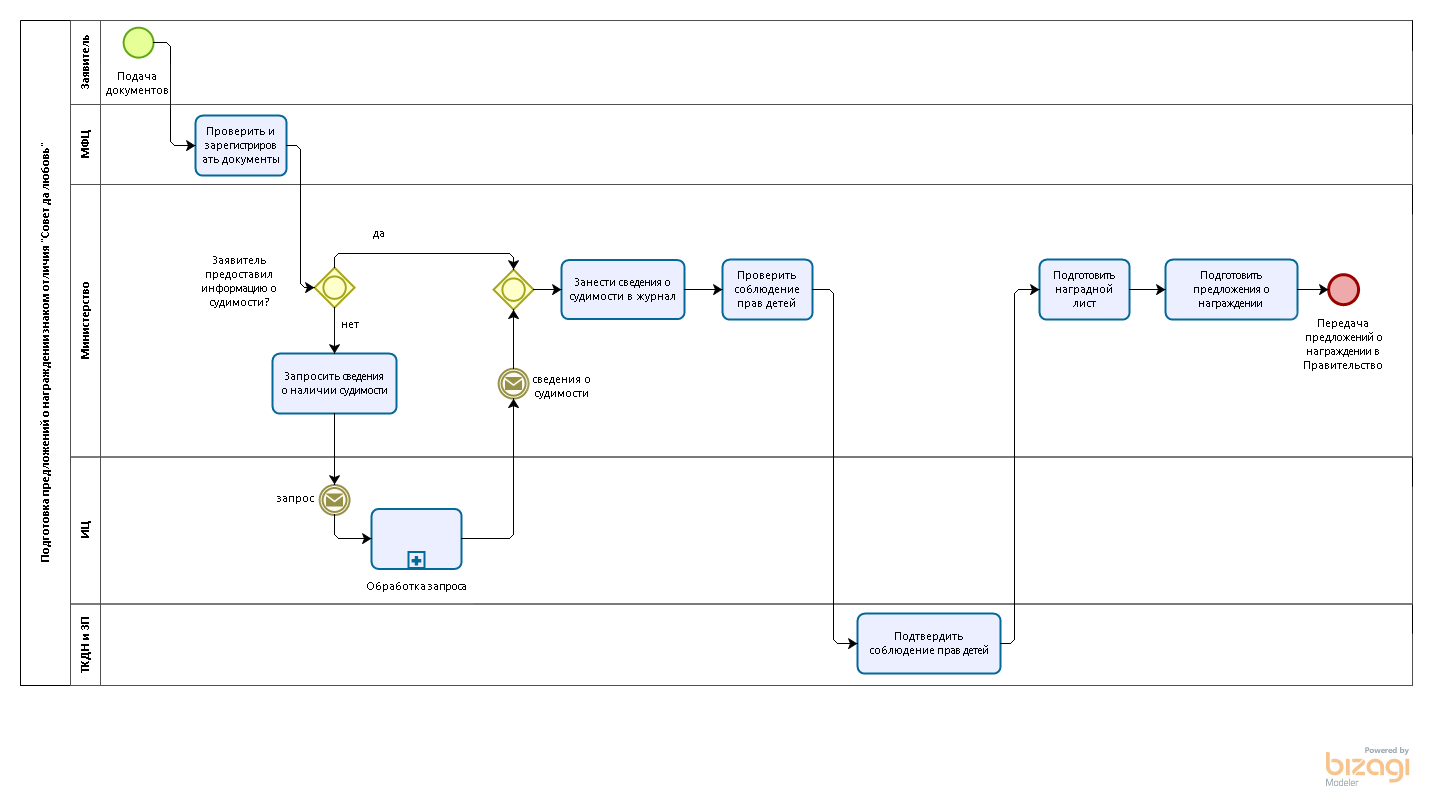
\includegraphics[width=\textwidth]{figures/model-description}
    \caption{Улуга <<Совет да любовь>> в нотации BPMN}
    \label{description}
\end{sidewaysfigure}

\clearpage
\section{Запуск моделирования}

Теперь, чтобы проверить корректность описания этапов нашего
процесса в нотации BPMN, мы можем запустить моделирование на
первом этапе (\textit{Process Validation}).

Для этого, нам нужно создать поток входных заявок в у
начального события, нажав на шестеренку рядом (Рис. \ref{run:flow}).
А также указать, в каком отношении соотносятся события,
происходящие на шлюзе (Рис. \ref{run:gate}): в нашем случае
мы считаем, что 90 \% заявителей не приносят сведения о судимости
при подачи заявления.
\myImage{Задание потока заявок на входе модели}{run_control}{run:flow}
\myImage{Задание вероятносного распределения на шлюзе}{run_if}{run:gate}
\clearpage

\myImage{Вывод отчета о проведенном моделировании}{run_report}{run:report}

Этого достаточно, чтобы запустить иммитацию процесса: перходим
в вид \textit{Simulation View} и нажимаем \textit{Run}.
В результате нам показывается отчет выполнения имитации (Рис. \ref{run:report}),
на котором мы видим количество пройденых заявок на каждом этапе.
Несмотря на большое количество согласований и проверок в нашем
процессе (проверка сведений о судимости, проверка соблюдения
прав детей), в регламенте услуги сказано, что нет никаких причин
в отказе оказания услуги, то есть она является этапом на котором
формируется вся необходимая информация. Поэтому количество
заявок на начальном событии должно быть равно количеству
заявок на конечном этапе, что выделено на рисунке.
Таким образом модель процесса составлена корректно.
